\bluepage{Model representation / Reprezentace modelu}

\begin{frame}
\frametitle{Input and Output Data / vstupní a výstupní data}
	\begin{itemize}
    \item{Main goal of the GPU is to conver 3D vector graphics to raster graphics (framebuffer)}
	\end{itemize}
	\begin{itemize}
    \item{Hlavním úkolem grafické karty je převod 3D vektorové grafiky na rastrový obrázek (framebuffer).}
	\end{itemize}
	\begin{figure}[h]
		
\includegraphics[width=10cm,keepaspectratio]{pics/model/vector2raster}
	\end{figure}
\end{frame}

\begin{frame}
\frametitle{Scene representation / Reprezentace scény}
	\begin{itemize}
    \item{Boundary representation (B-rep) - vector graphics.}
	\end{itemize}
	\begin{itemize}
		\item{Povrchová reprezentace - vektorová data.}
	\end{itemize}
	\begin{figure}[h]
		\includegraphics[width=10cm,keepaspectratio]{pics/model/wireframe.jpg}
	\end{figure}
\end{frame}

\begin{frame}
\frametitle{Scene representation / Reprezentace scény}
  \scriptsize
	\begin{itemize}
    \item{3D Vector graphics is not just points, lines and polygons.}
    \item{A GPU renders geometry based on vertices.}
    \item{A vertex is not just point in 3D space.}
    \item{A vertex is structure of user specific data.}
		\item{Jeden Vertex může obsahovat několik různých atributů (pozice, barva, čas, hmotnost, texturovací koordináty,...)}
		\item{Několik Vertexů tvoří jedno primitivum - bod, úsečka, trojúhelník,...}
	\end{itemize}

	\begin{itemize}
    \item{3D Vektorová grafika nejsou jen body, hrany a polygony.}
    \item{GPU kreslí geometrii založenou na vertexech.}
    \item{Vertex není jen bod v 3D prostoru.}
    \item{Vertex je struktura uživatelských dat.}
		\item{Jeden Vertex může obsahovat několik různých atributů (pozice, barva, čas, hmotnost, texturovací koordináty,...)}
		\item{Několik Vertexů tvoří jedno primitivum - bod, úsečka, trojúhelník,...}
	\end{itemize}
	\begin{figure}[h]
		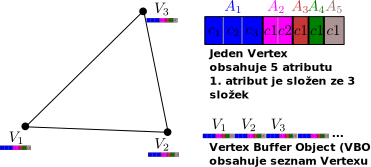
\includegraphics[width=9cm,keepaspectratio]{pics/model/primitive.pdf}
	\end{figure}
\end{frame}

\begin{frame}
\frametitle{Geometry terminology / Geometrická terminologie}
  \scriptsize
  The scene is usually composed using:
	\begin{itemize}
    \item{A scene graph - user friendly, hierarchical structure of the scene.}
    \item{A model - one object of the scene. Can be instanced.}
    \item{A mesh - one piece of model. 1 material, 1 kind of geometry.}
    \item{A primitive - geometric piece, 2 categories: base primitives (point, line, triangle) and primimitive.}
    \item{A vertex - structure of user specific vertex attributes (data).}
		\item{A vertex attribute - 1-4D vector of floats or integers.}
    \item{A vertex buffer - memory containing vertices.}
    \item{A element/index buffer - memory containing indices to vertices.}
	\end{itemize}

  Scéna je obvykle složena z:
	\begin{itemize}
    \item{Graf scény - uživatelsky přívětivá hierarchická struktura scény.}
    \item{Model - jeden objekt scény, který je možné instanciovat.}
    \item{Mesh - jeden kousek modelu, obvykle má jen jeden materiál a jeden typ geometrie.}
    \item{Primitivum - geometrický kousek, dvě kategorie: základní primitiva (bod, úsečka, trojúhelník) a primitiva.}
    \item{Vertex - struktura uživatelských vertex atributů (data).}
		\item{Vertex atribut - 1-4 dimenzionální vektor floatů nebo integerů.}
    \item{Vertex Buffer - paměť obsahující vrcholy.}
    \item{Index/Element buffer - paměť obsahující indexy na vrcholy.}
	\end{itemize}
\end{frame}


\begin{frame}
\frametitle{Base Primitives / Základní primitivum}
  \scriptsize

	\begin{itemize}
    \item{The base primitive is subset of all primitives. There are only 3 types - triangles, lines, points. There is specialized rasterization hardware for each type. More complex primitives are composed of these base primitives.}
	\end{itemize}

	\begin{itemize}
    \item{Záklaní primitiva tvoří podmnožinu všech primitiv. Jsou jen tři typy (trojúhelník, úsečka, bod). Pro každý je rasterizační hardware. Složitější primitiva jsou z nich složena.}
	\end{itemize}
	\begin{figure}[h]
		
\includegraphics[width=9cm,keepaspectratio]{pics/model/base_prim.pdf}
	\end{figure}
\end{frame}

\begin{frame}
\frametitle{Common Primitives / Běžná primitiva}
  \scriptsize

	\begin{itemize}
    \item{Base primitives together with these primitives form commonly used primitives. Main purpose is to reduce memory footprint and processing time.}
	\end{itemize}

	\begin{itemize}
    \item{Kromě základních primitiv se ještě běžně používají tato primitiva. Hlavním účelem je ušetřit paměť a čas zpracování.}
	\end{itemize}
	\begin{figure}[h]
		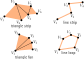
\includegraphics[width=9cm,keepaspectratio]{pics/model/common_prim.pdf}
	\end{figure}
\end{frame}

\begin{frame}
\frametitle{Primitives with adjacency / Primitiva se sousedností}
  \scriptsize

	\begin{itemize}
    \item{There are also primitives with adjacency (mainly for geometry shader).}
	\end{itemize}

	\begin{itemize}
    \item{Existují také primitiva se sousedností (hlavně pro geometry shader).}
	\end{itemize}
	\begin{figure}[h]
		
\includegraphics[width=10cm,keepaspectratio]{pics/model/prim_adjacency.pdf}
	\end{figure}
\end{frame}
